\documentclass{classrep}
\usepackage[utf8]{inputenc}
\usepackage{graphicx}
\usepackage{color}
\usepackage{caption} % opcjonalnie, dla lepszego formatowania

\DeclareUnicodeCharacter{00A0}{~}

\studycycle{Informatyka, studia dzienne, inż I st.}
\coursesemester{IV}

\coursename{Sztuczna inteligencja i systemy ekspertowe}
\courseyear{2024/2025}

\courseteacher{Dr. inż. Krzysztof Lichy}
\coursegroup{wtorek, 12:00}

\author{
  \studentinfo{Mikołaj Pawłoś}{258681} \and
  \studentinfo{Emilia Szczerba}{251643}
}

\title{Zadanie drugie: Poprawa lokalizacji UWB przy pomocy sieci neuronowych}

\begin{document}
\maketitle

\section{Cel}
 {Zaprojektowanie i zaimplementowanie sieci neuronowej,
  która pozwoli na korygowanie błędów uzyskanych z systemu pomiarowego.}


\section{Wprowadzenie}
\paragraph{}
\textbf{Sieć neuronowa} (znana również jako \textit{sztuczna sieć neuronowa},
w skrócie \textbf{NN} lub \textbf{ANN})
to model obliczeniowy inspirowany strukturą i funkcjami biologicznych sieci neuronowych.
Sieć neuronowa składa się z połączonych jednostek lub węzłów, zwanych \textbf{sztucznymi neuronami}, które luźno odwzorowują neurony w mózgu.
\paragraph{}
\textbf{Neurony} są połączone \textbf{krawędziami}, które odwzorowują synapsy w mózgu. Każdy sztuczny neuron odbiera sygnały od połączonych z nim neuronów, przetwarza je, a następnie wysyła sygnał do kolejnych połączonych neuronów.
\paragraph{}
„\textbf{Sygnał}” ma postać liczby rzeczywistej, a wyjście neuronu obliczane jest
za pomocą pewnej nieliniowej funkcji sumy jego wejść, zwanej \textbf{funkcją aktywacji}.
\paragraph{}
Siła sygnału w każdym połączeniu jest określana przez \textbf{wagę}, która jest dostosowywana podczas procesu uczenia.

Zazwyczaj neurony grupowane są w \textbf{warstwy}. Różne warstwy mogą wykonywać różne transformacje danych wejściowych.
Sygnały przepływają od pierwszej warstwy (\textit{warstwa wejściowa}) do ostatniej (\textit{warstwa wyjściowa}),
przechodząc być może przez kilka warstw pośrednich (\textit{warstw ukrytych}).
Sieć nazywa się \textbf{głęboką siecią neuronową}, jeśli zawiera co najmniej dwie warstwy ukryte.

\begin{figure}[h!]
	\centering
	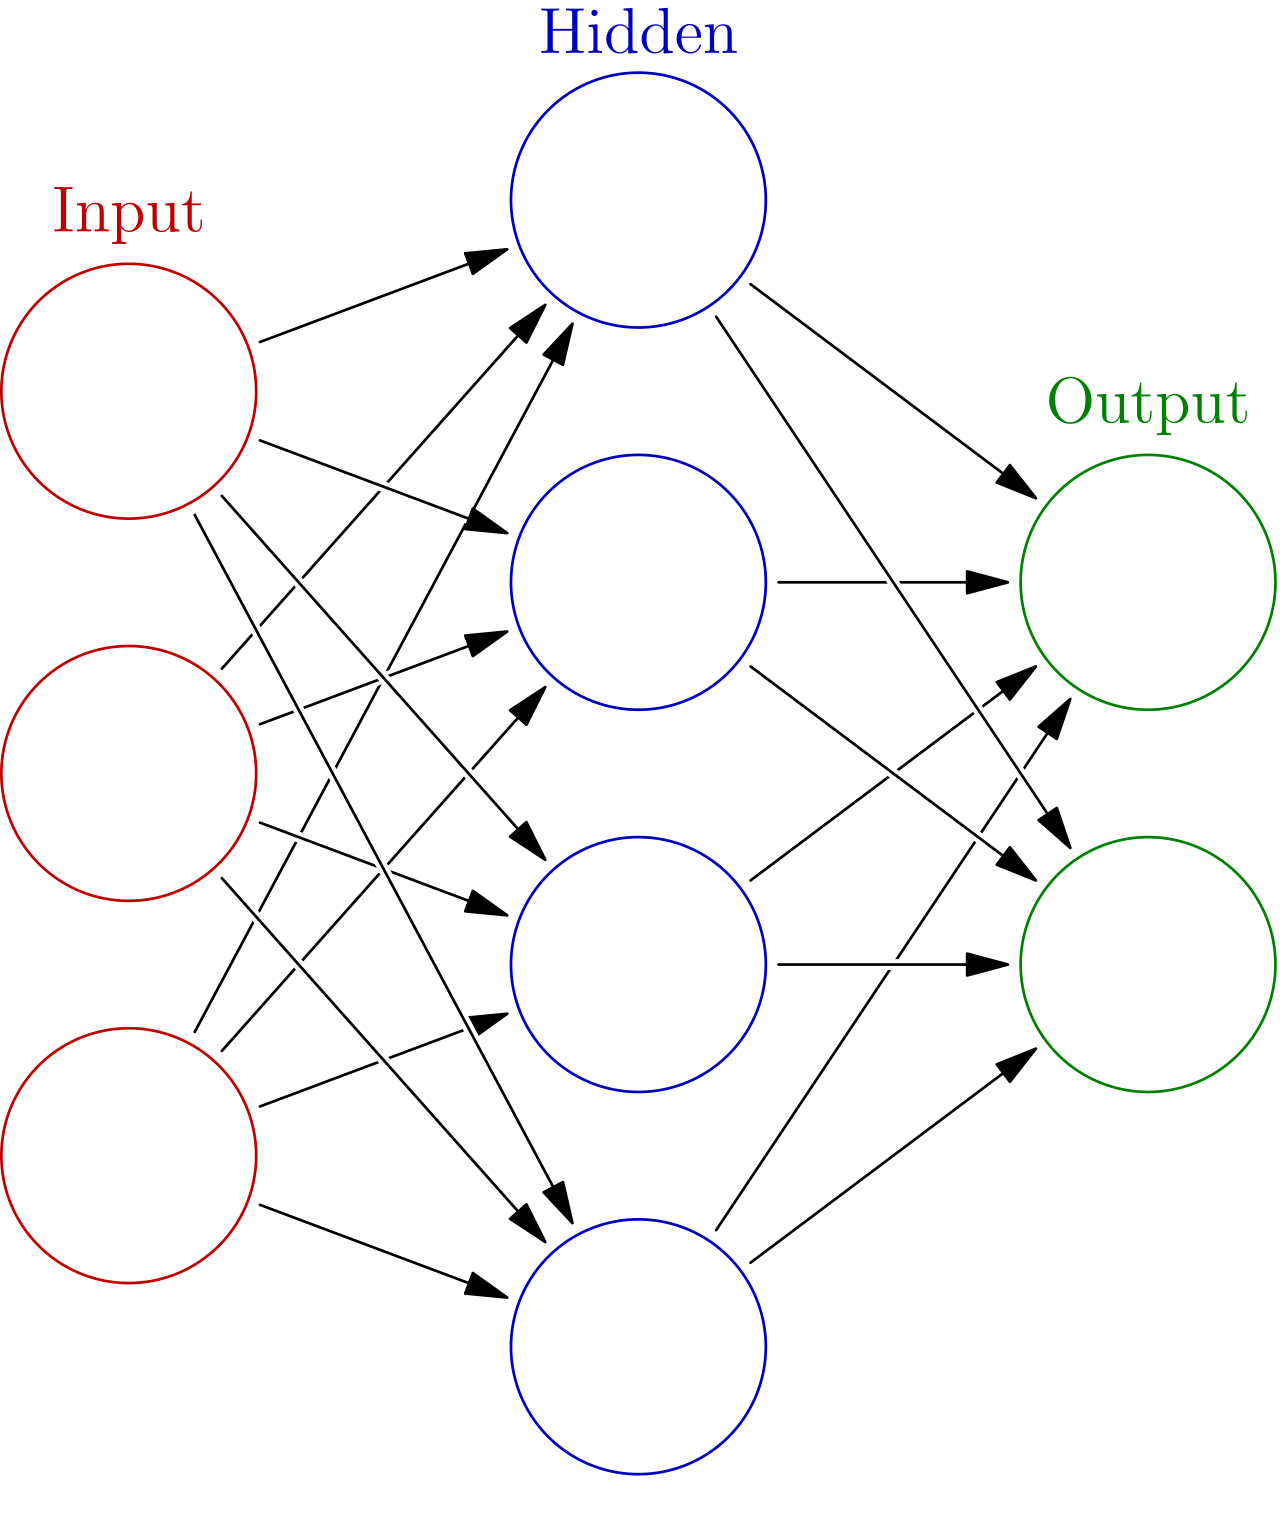
\includegraphics[scale=0.2]{nn.png}
	\caption{Schemat przykładowej sieci neuronowej}
	\label{fig:nn}
\end{figure}

Sztuczne sieci neuronowe są wykorzystywane w różnych zadaniach, takich jak \textit{modelowanie predykcyjne}, \textit{sterowanie adaptacyjne} czy \textit{rozwiązywanie problemów z zakresu sztucznej inteligencji}. Potrafią uczyć się na podstawie doświadczenia i wyciągać wnioski z złożonych i pozornie niepowiązanych danych.

\clearpage{}
\section{Opis implementacji}

Zadanie zostało wykonane przy użyciu języka \textbf{Python3}, z wykorzystaniem następujących bibliotek:

\begin{itemize}
	\item \texttt{Matplotlib}
	\item \texttt{Numpy}
	\item \texttt{PyTorch}
	\item \texttt{scikit-learn}
\end{itemize}

Projekt został podzielony na następujące pliki:

\begin{enumerate}
	\item \texttt{DataLoader.py} – moduł odpowiedzialny za wczytywanie, filtrowanie i wstępne przetwarzanie danych pomiarowych z plików Excel.

	\item \texttt{NeuralNetworkModel.py} – główny moduł modelu uczenia maszynowego opartego na sieci neuronowej. Odpowiada za tworzenie, trenowanie, testowanie i zapisywanie modelu, z uwzględnieniem mechanizmów detekcji outlierów i normalizacji danych.

	\item \texttt{OutlierDetector.py} – moduł odpowiedzialny za identyfikację obserwacji odstających w danych wejściowych. Wspiera różne metody detekcji, m.in. oparte na odległości Mahalanobisa czy odchyleniu standardowym.

	\item \texttt{main.py} – plik uruchomieniowy, zawierający konfigurację eksperymentów, wczytywanie danych, inicjalizację modelu oraz zapisywanie wyników i metryk. Stanowi punkt wejścia do całego systemu.

\end{enumerate}

\clearpage{}
\subsection{Plik \texttt{DataLoader.py}}

Moduł \texttt{DataLoader.py} odpowiada za ładowanie oraz wstępne przetwarzanie danych pomiarowych wykorzystywanych w procesie uczenia i testowania modeli.
Główne zadania realizowane przez ten moduł to:

\begin{itemize}
	\item automatyczne lokalizowanie folderów z danymi wejściowymi (statycznymi i dynamicznymi),
	\item odczyt danych z plików Excel (\texttt{.xlsx}) znajdujących się w podfolderach \texttt{F8} i \texttt{F10},
	\item wstępne czyszczenie danych – usuwanie pustych wierszy,
	\item selekcja i ekstrakcja cech sensorycznych z kolumn (np. akcelerometr, żyroskop, ciśnienie, kwaterniony),
\end{itemize}

Dane są dzielone na zbiór treningowy (pochodzący z plików statycznych) oraz testowy (z plików dynamicznych), a następnie przekształcane do postaci numerycznych macierzy przy pomocy biblioteki NumPy.
Moduł ten stanowi fundament do dalszych etapów analizy i modelowania, zapewniając jednolite i ustandaryzowan

\subsection{Plik \texttt{NeuralNetworkModel.py}}

Plik \texttt{NeuralNetworkModel.py} zawiera kompletną implementację modelu sieci neuronowej zaprojektowanej z myślą o regresji wielowymiarowej oraz automatycznej detekcji i eliminacji obserwacji odstających (ang. outliers).

Moduł składa się z dwóch głównych klas:
\begin{itemize}
	\item \texttt{NeuralNetwork} – definiuje architekturę wielowarstwowej sieci neuronowej typu \textit{feedforward} z konfigurowalną liczbą warstw ukrytych, funkcją aktywacji i mechanizmem \texttt{Dropout}.
	\item \texttt{EnhancedNeuralNetworkModel} – klasa wyższego poziomu integrująca funkcje uczenia, walidacji, normalizacji danych, predykcji oraz obsługi danych odstających przy użyciu zewnętrznego modułu \texttt{OutlierDetector}.
\end{itemize}

Model wspiera różne optymalizatory (Adam, SGD), posiada wbudowany mechanizm \textit{early stopping}, adaptacyjny harmonogram uczenia (\texttt{ReduceLROnPlateau}) oraz możliwość zapisu i odczytu wag modelu (zarówno w formacie binarnym \texttt{.pt}, jak i w postaci tabeli CSV).

Trening odbywa się z użyciem biblioteki PyTorch, a dane wejściowe są wstępnie przeskalowywane za pomocą standaryzacji (\texttt{StandardScaler}) z biblioteki \texttt{scikit-learn}. Proces walidacji może być przeprowadzony na osobnym zbiorze lub automatycznie podzielony z danych treningowych.

Architektura modelu jest w pełni parametryzowana: użytkownik może zdefiniować liczbę neuronów wejściowych, wyjściowych, strukturę warstw ukrytych, liczbę epok, współczynnik uczenia, funkcję aktywacji, metodę detekcji outlierów, a także urządzenie obliczeniowe (\texttt{CPU} lub \texttt{GPU}).

\pagebreak
\subsection{Plik \texttt{OutlierDetector.py}}

Moduł \texttt{OutlierDetector.py} zawiera klasę \texttt{OutlierDetector}, która odpowiada za identyfikację oraz usuwanie odstających obserwacji (ang. \textit{outliers}) w danych wejściowych i wyjściowych modeli regresyjnych. Celem tego modułu jest poprawa jakości danych poprzez eliminację punktów, które mogą negatywnie wpłynąć na proces uczenia lub predykcji.

\paragraph{}
\textbf{Obsługiwane metody detekcji outlierów}:
\begin{itemize}
	\item \textbf{Z-score} – klasyczna metoda statystyczna oparta na standaryzacji zmiennych i analizie ich odchyleń od średniej.
	\item \textbf{IQR (Interquartile Range)} – metoda oparta na analizie rozstępu międzykwartylowego (dolna i górna granica = $Q1 - 1.5 \cdot IQR$, $Q3 + 1.5 \cdot IQR$).
	\item \textbf{Isolation Forest} – metoda oparta na modelu lasu losowego izolującego punkty anomalne.
	\item \textbf{Odległość Mahalanobisa} – metoda uwzględniająca współzmienność danych i odległość od centroidu wielowymiarowego.
	\item \textbf{Combined} – strategia łącząca wyniki trzech metod (Z-score, IQR, Mahalanobis); punkt uznawany jest za outlier, jeśli zostanie wykryty przez co najmniej dwie z nich.
\end{itemize}

\paragraph{}
\textbf{Kluczowe cechy klasy \texttt{OutlierDetector}}:
\begin{itemize}
	\item Obsługuje brakujące dane (NaN, inf) poprzez ich czyszczenie lub zastępowanie medianą.
	\item Uwzględnia błędy obliczeń numerycznych (np. osobliwość macierzy kowariancji).
	\item Zawiera system awaryjny: w przypadku błędu w jednej metodzie, automatycznie używana jest metoda Z-score jako domyślna.
	\item Dostarcza pełną analizę statystyczną: liczba wykrytych outlierów, procentowy udział oraz rozmiar zbioru po filtracji.
\end{itemize}

\paragraph{}
\textbf{Główne metody klasy}:
\begin{itemize}
	\item \texttt{detect\_outliers\_zscore(data, threshold)} – detekcja przy użyciu standaryzacji i progu odcięcia.
	\item \texttt{detect\_outliers\_iqr(data)} – detekcja oparta na kwartylach.
	\item \texttt{detect\_outliers\_isolation\_forest(data)} – detekcja z wykorzystaniem modelu \texttt{IsolationForest}.
	\item \texttt{detect\_outliers\_mahalanobis(data)} – detekcja w oparciu o wielowymiarową odległość Mahalanobisa.
	\item \texttt{detect\_outliers(X, Y)} – metoda główna, wykonująca detekcję na połączonych danych wejściowych i wyjściowych.
	\item \texttt{filter\_data(X, Y)} – zwraca przefiltrowane dane z usuniętymi outlierami.
	\item \texttt{outlierDetector(X, Y)} – metoda pomocnicza, kompatybilna z interfejsem używanym w kodzie sieci neuronowej.
\end{itemize}

\paragraph{}
Moduł umożliwia elastyczne dostosowanie metody detekcji poprzez parametr \texttt{method} podawany w konstruktorze. Dodatkowo zastosowano szeroko zakrojone zabezpieczenia przed nieoczekiwanym zachowaniem danych, w tym sprawdzanie ich poprawności, kształtów, oraz odpowiednie logowanie przebiegu przetwarzania.


\section{Materiały i metody}
 {\color{blue}
  W tym miejscu należy opisać, jak przeprowadzone zostały wszystkie badania,
  których wyniki i dyskusja zamieszczane są w dalszych sekcjach. Opis ten
  powinien być na tyle dokładny, aby osoba czytająca go potrafiła wszystkie
  przeprowadzone badania samodzielnie powtórzyć w celu zweryfikowania ich
  poprawności. Przy opisie należy odwoływać się i stosować do
  opisanych w sekcji drugiej wzorów i oznaczeń, a także w jasny sposób opisać
  cel konkretnego testu. Najlepiej byłoby wyraźnie wyszczególnić (ponumerować)
  poszczególne eksperymenty tak, aby łatwo było się do nich odwoływać dalej.}

\section{Wyniki}
 {\color{blue}
  W tej sekcji należy zaprezentować, dla każdego przeprowadzonego eksperymentu,
  kompletny zestaw wyników w postaci tabel, wykresów (preferowane) itp. Powinny
  być one tak ponazywane, aby było wiadomo, do czego się odnoszą. Wszystkie
  tabele i wykresy należy oczywiście opisać (opisać co jest na osiach, w
  kolumnach itd.) stosując się do przyjętych wcześniej oznaczeń. Nie należy tu
  komentować i interpretować wyników, gdyż miejsce na to jest w kolejnej sekcji.
  Tu również dobrze jest wprowadzić oznaczenia (tabel, wykresów), aby móc się do
  nich odwoływać poniżej.}

\section{Dyskusja}
 {\color{blue}
  Sekcja ta powinna zawierać dokładną interpretację uzyskanych wyników
  eksperymentów wraz ze szczegółowymi wnioskami z nich płynącymi. Najcenniejsze
  są, rzecz jasna, wnioski o charakterze uniwersalnym, które mogą być istotne
  przy innych, podobnych zadaniach. Należy również omówić i wyjaśnić wszystkie
  napotkane problemy (jeśli takie były). Każdy wniosek powinien mieć poparcie we
  wcześniej przeprowadzonych eksperymentach (odwołania do konkretnych wyników).
  Jest to jedna z najważniejszych sekcji tego sprawozdania, gdyż prezentuje
  poziom zrozumienia badanego problemu.}

\section{Wnioski}
 {\color{blue}
  W tej, przedostatniej, sekcji należy zamieścić podsumowanie najważniejszych
  wniosków z sekcji poprzedniej. Najlepiej jest je po prostu wypunktować. Znów,
  tak jak poprzednio, najistotniejsze są wnioski o charakterze uniwersalnym.}

\begin{thebibliography}{0}
	\bibitem{l2short} Wikipedia contributors. "Neural network (machine learning)."
	Wikipedia, The Free Encyclopedia. Wikipedia, The Free Encyclopedia,
	29 May. 2025. Web. 29 May. 2025. \end{thebibliography}

{\color{blue}
Na końcu należy obowiązkowo podać cytowaną w sprawozdaniu literaturę, z której
grupa korzystała w trakcie prac nad zadaniem.}

\end{document}
